\documentclass{article}
\usepackage{graphicx}
\usepackage{amsmath,amssymb}
\setlength{\parindent}{0pt}
\usepackage{listings}
\usepackage{lmodern}  % for bold teletype font
\usepackage{amsmath}  % for \hookrightarrow
\usepackage{xcolor}   % for \textcolor
\usepackage[a4paper,margin=1in,footskip=0.25in]{geometry}
\usepackage{graphicx}

\lstset{
  basicstyle=\ttfamily,
  columns=fullflexible,
  frame=single,
  breaklines=true,
}

\begin{document}

\title{Deep Reinforcement Learning Project 2 : Continuous Control}
\author{Rachel Schlossman}

\maketitle

\section{Learning Algorithm}
The learning algorithm is a modified implementation of the Deep Deterministic Policy Gradient (DDPG) algorithm \cite{lillicrap2015continuous} in order to be applicable to multi-agent reinforcement learning. It is important to note how this implementation is different from the multi-agent Deep Deterministic Policy Gradient (MADDPG) algorithm as described in \cite{lowe2017multi}. As the referenced paper describes, the algorithm is based on (1) each agent having its own actor network to approximate the actor function (decentralized exection) and (2) a centralized critic network with access to all agents' observations and actions (centralized learning). In contrast to this, the algorithm in this project leverages a single actor network and a single critic network (centralized execution and learning). The two networks are shared between the two agents; The actor network only has access to a single agent's observations and, similarly, the critic only has access to a single agent's observations and actions. So, at a single timestep, the same network parameters are used to devise both agents' policies and action-value functions. This strategy is appropriate for the Tennis environment because the environment is symmetric; the agents have the same observations, actions, and reward function; and neither agent is rewarded directly for beating the other agent.


\subsection{Hyperparameters}
The following hyperparameters were used in the implementation:

\begin{itemize}
\item replay buffer size : 1e6
\item minibatch size: 128
\item discount factor: 0.99 
\item for soft update of target parameters, $\tau$: 1e-3
\item learning rate of the actor: 1e-4  
\item learning rate of the critic: 1e-4 
\item L2 weight decay: 0
\end{itemize}


\section{Model Architecture}
The modified DDPG algorithm employs two neural networks, the actor network and the critic network. For both networks, the input passes through two linear layers with relu activation. For the actor network the input is the observation (length 24) and the hidden layers are followed by a tanh output layer. For the critic network, the input is also the observation, and in the first hidden layer the (length 2) action is appended to the input layer's outputs. The hidden layers are followed by a linear output layer. The two hidden layers  for each network each are comprised of 256 nodes (excluding the concatenation of the actions).  

\section{Results}
The two agents are able to receive an average reward (over 100 episodes, and over all both agents) of at least 0.5 in 2406 episodes, as shown in Figure \ref{fig:results}.

\begin{figure}[ht]
\centering
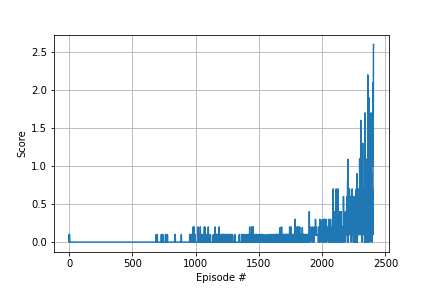
\includegraphics[scale=0.75]{../implementation/figures/results.png}
\caption{Average Score Plot}
\label{fig:results}
\end{figure}

\section{Future Work}
In the future it would be of interest (1) to explore learning behavior via a prioritized replay buffer and (2) to implement decentralized policy execution via two separate action networks, one per agent. 

\bibliographystyle{plain}
\bibliography{bib}




\end{document}